\documentclass[12pt]{article}

\title{Password-Based Authentication with Zero-Knowledge Proof of Quadratic Residuosity}
\author{Jakob Povsic}
\date{2020}

\usepackage{listings}
\usepackage{amsmath}
\usepackage{tgschola}
\usepackage{amsfonts}
\usepackage{mathptmx}
\usepackage{graphicx}
\usepackage{hyperref}

\fontfamily{qcs}

\newcommand{\Mod}[1]{\ (\mathrm{mod}\ #1)}

\renewcommand{\thefootnote}{\fnsymbol{footnote}}
\newcommand{\genlegendre}[4]{%
  \genfrac{(}{)}{}{#1}{#3}{#4}%
  \if\relax\detokenize{#2}\relax\else_{\!#2}\fi
}
\newcommand{\legendre}[3][]{\genlegendre{}{#1}{#2}{#3}}
\newcommand{\dlegendre}[3][]{\genlegendre{0}{#1}{#2}{#3}}
\newcommand{\tlegendre}[3][]{\genlegendre{1}{#1}{#2}{#3}}

\begin{document}
\pagenumbering{Roman}

\maketitle
\newpage

\tableofcontents
\newpage

\pagenumbering{arabic}

\section{Abstract}
In this thesis I will introduce the notion of zero-knowledge proofs, their variants and formal definitions.
In the second part of the thesis I will present a protocol for password based authentication based on the zero-knowledge proof of quadratic residuosity.
In the last part of the thesis I will document the implementation of the protocol as an EAP authentication method.

\section{Introduction}
Something about how privacy and security are becoming ever more important as our world is becoming ever more digitalised and connected.

\subsection{Example}

A famous example of a zero-knowledge proof protocol made by \cite{QJM} is The Strange Cave of Ali Baba.

\bigskip

Ali Baba's cave is a cave with a single entrance, that splits into two tunnels that meet in the middle. Where the tunnels meet is a door that can only be opened with a secret passphrase.

\bigskip

Peggy\footnote{Peggy is acronym for \textbf{Prover}} wants to prove to Victor \footnote{Victor is an acronym for \textbf{Verifier}} that she knows the secret passphrase, but she doesn't want to revel the secret nor does she want to reveal her knowledge of the secret to anyone else besides 

\bigskip

Victor turns away from the entrance of the cave, so he cannot Peggy. Peggy enters the cave and goes into one of the tunnels at random. Victor turns around and tells Peggy which tunnel to come out of. Peggy knowing the secret can pass through the door in the middle and emerge from the tunnel requested by Victor.

\bigskip

Given that Peggy didn't know the secret she would still be able to emerge from the tunnel that she initially entered if Victor requested it. Since Victor is choosing the tunnel at random, Peggy has 50\% chance of entering the correct tunnel, and by repeating this process her chances of cheating become vanishingly small ($\frac{1}{2^n}$).

Inversely if Peggy emerges from tunnels Victor requests, he can be convinced that Peggy knows the secret passphrase with a very high probability ($1 - \frac{1}{2^n}$).

\bigskip

Further more any third party observing the interaction cannot be convinced of the validity of the proof because it cannot be assured that the interaction was truly random. For example, Victor could have told Peggy his questions in advance, so Peggy would produce a convincing looking proof.

\section{Zero-Knowledge Proofs}

Traditional theorem proofs are logical arguments that establish truth through inference rules of a deductive system based on axioms and other proven theorems.
\textit{Zero-Knowledge Proofs} (ZKPs) are compared to traditional proofs probabilistic meaning they \textit{"convince"} the verifier with a small margin of error.

They were first defined by Goldwasser, Micali and Rackoff in \cite{GMR} in a paper published in 1985. 
They proposed a proof system as a two-party protocol between a \textit{prover} and a \textit{verifier}. 
It relies on the computational difficulty of the quadratic residuosity problem (QRP).

%There are three main ingredients that make interactive zero-knowledge proofs work. %TODO: Move this part to the end of the section
%
%\begin{enumerate}
%	\item Interaction - The prover and the verifier exchange messages back and forth.
%	\item Hidden Randomisation - The verifier relies on randomness that is hidden from the prover, and thus unpredictable from him.
%	\item Computational Difficulty - The prover embeds his proof in computational difficulty of some other problem.
%\end{enumerate}

\subsection{Interactive Proof Systems}
\textbf{Interactive proof systems} are proof systems between a prover and a verifier, which exchange messages to decide on the validness of the proof.
The prover is a computationally unbounded polynomial time Turing machine and the verifier is a probabilistic polynomial time Turing machine.


The properties of \textit{completeness} and \textit{soundness} define an interactive proof system.

\paragraph{Completeness}

Any honest prover can convince the verifier with overwhelming probability.\\
For each $k \in \mathbb{N}$ and sufficiently large $n$;

$$\Pr[x \in L; P(x) = y; V(y) = 1] \ge 1 - \frac{1}{n^k}$$

\paragraph{Soundness}

Any verifier following the protocol will reject a cheating prover with overwhelming probability.\\
For each $k \in \mathbb{N}$ and sufficiently large $n$;

$$\Pr[x \notin L; P(x) = y; V(y) = 0] \ge 1 - \frac{1}{n^k}$$


\subsubsection{Interactive Polynomial Time Complexity}
Any problem solvable by an interactive proof systems is in the class of \textbf{IP}.

\subsubsection{Other Variants of Interactive Proof Systems}

\paragraph{Arthur-Merlin protocol} Problems in the class \textbf{AM}, an Arthur-Merlin protocol \cite{babai1985trading} is an interactive protocol similar to IP, with the difference in that its a \textit{public-coin protocol}. 
Meaning that verifiers internal state is visible to the prover, while in IP the state is hidden.
%I has been proven that AM is equally powerful as IP and that AM's public internal state gives the prover no advantage. %TODO: Add citation

\paragraph{Multi Prover Interactive Proofs}
\textbf{MIP} \cite{ben2019multi} is a more powerful model, utilising two provers that communicate with a single verifier.
This models has been build to address the shortcomings of IP.
MIP proved that every problem has a ZKP system, without the assumption that one-way functions exist.

\subsection{Knowledge Complexity}

\textit{Zero-knowledge proof systems} prove the  membership of $x$ in language $L$, without revealing any additional knowledge (e.g why is $x \in L$).

The essence of zero-knowledge is the idea that what the verifier \textit{sees} is indistinguishable from what can be easily \textit{simulated} on public inputs.
The term \textit{knowledge complexity} quantifies the degrees of indistinguishability of different languages and proof constructions. 

\subsubsection{Indistinguishability}
Indistinguishability describes degrees of an ability to distinguish between two random variables $U, V$.
\bigskip
\newline
Let $U = \{U(x)\}$ and $V = \{V(x)\}$ be two families of random variables, where $x$ is from a language $L$, a subset of $\{0, 1\}^*$.
\newline
An algorithm $A(x)$ is given a random sample $x$ from either distribution and will output either $1$ or $0$, depending which distribution it determines the sample originated from.
Distributions become "indistinguishable" as the outputs of the algorithm become uncorrelated to the origin of the sample.

By bounding the \textit{size} of the sample and the \textit{time} given to the algorithm we can obtain different notions of indistinguishability.

%\subsubsection{Indistinguishability of Random Variables} %TODO: Simplify this
%
%Let $U = \{U(x)\}$ and $V = \{V(x)\}$ be two families of random variables, where $x$ is from a language $L$, a particular subset of $\{0, 1\}^*$.
%
%In the framework for distinguishing between random variables, a "judge" is given a sample selected randomly from either $V(x)$ or $U(x)$.
%A judge studies the sample and outputs either a $0$ or a $1$, depending on which distribution he thinks the sample came from.
%
%$U(x)$ essentially becomes "replaceable" by $V(x)$, when $x$ increases and any judges prediction becomes uncorrelated with the origin distribution.


\paragraph{Equality} 
%Given that $U(x)$ and $V(x)$ are equal, they will remain indistinguishable, even if the samples are of arbitrary size and can be studied for an arbitrary amount of time.

If $U(x)$ and $V(x)$ are equal, outputs of a computationally unbounded algorithm will remain uncorrelated with the origin of the sample.

\paragraph{Statistical Indistinguishability} Two random variables are statistically indistinguishable, when the algorithms outputs remain uncorrelated with the origin, given an arbitrary amount of time and a poly-bounded sample size.
\bigskip
\newline
Let $L \subset \{0,1\}^*$ be a language, $U(x)$ and $V(x)$ are statistically indistinguishable on $L$ if,
\bigskip
$$|\Pr [A(x, U) = 1] - \Pr [A(x, V) = 1]| < |x|^{-c}$$ %TODO: Probably not right, check later.
\bigskip
\newline
for $\forall c > 0$, and sufficiently long $x \in L$. 

%\subparagraph{Statistical Indistinguishability} Two random variables are statistically indistinguishable, when given a polynomial sized sample and an arbitrary amount of time, the judges verdict remains meaningless.
%
%\bigskip
%
%Let $L \subset \{0,1\}^*$ be a language, $U(x)$ and $V(x)$ are statistically indistinguishable on $L$ if,
%
%$$\sum_{\alpha \in \{0,1\}^*} |prob(U(x) = \alpha) - prob(V(x) = \alpha) | < |x|^{-c}$$
%
%
%
%for $\forall c > 0$, and sufficiently long $x \in L$. 

\paragraph{Computational Indistinguishability} %TODO: Probably need to clarify the link between poly-time algorithm and poly-sized family of circuits.
Two random variables are computationally indistinguishable, when the poly-time bounded algorithms outputs remain uncorrelated with the origin, given a poly-bounded sample size.
\bigskip
\newline
Let $L \subset \{0,1\}^*$ be a language, poly-bounded families of random variables $U(x)$ and $V(x)$ are computationally indistinguishable on $L$ if for all poly-sized family of circuits $C$, $\forall c > 0$, and a sufficiently long $x \in L$

$$|\Pr[C(U, x) = 1] - \Pr[C(V, x) = 1]|  < |x|^{-c}$$


%\subparagraph{Computational Indistinguishability}%TODO: Simplify this
%
%Two random variables are computationally indistinguishable, if judges verdict remains meaningless given a polynomial sized sample and polynomial amount of time.
%
%\bigskip
%
%Let $L \subset \{0,1\}^*$ be a language, poly-bounded families of random variables $U(x)$ and $V(x)$ are computationally indistinguishable on $L$ if for all poly-sized family of circuits $C$, $\forall c > 0$, and a sufficiently long $x \in L$
%
%$$|P(U, C, x) - P(V, C, x)| < |x|^{-c}$$
%
%Any two families that are \textit{computationally indistinguishable} are considered  \textit{indistinguishable} in general.

\subsubsection{Approximability of Random Variables}%TODO: Simplify this

The notion of approximability described the degree to which a random variable $U(x)$ can be "generated" by a probabilistic Turing machine $M$, generating a probability distribution $M(x)$.
\bigskip
\newline
A random variable $U(x)$ is \textit{perfectly approximable} if there exists a probabilistic Turing machine $M$, such that for $x \in L$, $M(x)$ is \textit{equal} to $U(x)$.
\newline
$U(x)$ is statistically or computationally approximable if $M(x)$ is statistically or computationally indistinguishable from $U(x)$.

\bigskip

Generally speaking when saying a family of random variables $U(x)$ is \textit{approximable} we mean that it is \textit{computationally} approximable.

\subsubsection{Definition of Zero-Knowledge}

Zero-knowledge is a degree of protocols knowledge complexity at which no meaningful information can be extracted by the verifier or any third party observer.
\bigskip
\newline
A protocol is zero-knowledge if the verifiers "view" is approximable by a simulator $S$.
A verifiers view is all data that was exchanged with the prover, a cheating verifier's view might have extra information (e.g a history of previous interactions).

A protocols is perfectly zero-knowledge if the view is perfectly approximable for all verifiers.
Statistical or computational zero-knowledge is obtained by statistical or computational approximability.
\section{Languages with Zero-Knowledge Proof Systems}

One of the main components that make Zero-Knowledge proofs work is the encoding of the proof in the \textit{solution} of another "problem". The choice of the "problem" heavily relies on the specific application of the ZKP protocol. %TODO: Bullshit remove

A theoretical term from the computational complexity theory for a "problem" is \textit{language}. And the "problem" is the task of proving the membership of $x$ in language $L$ %TODO: Bullshit remove
%TODO: should be an introduction in the section
\\
\\
\\
Alongside specific languages with ZKPs, they have been also studies related to classes of languages defined by their computational complexity. %TODO: Also as a tool to study complexity, find sources.

In this thesis we are focusing on the zero-knowledge proof of quadratic residuosity, but generally ZKP protocols exists for any language in NP \cite{GMW}, assuming one way-functions exist in IP\footnote{Class of problems solved by an \textit{interactive proof system}}

%TODO: Mention other languages: GISO, DLOG

\subsection{Quadratic residuosity problem}

The original ZKP protocol described in \cite{GMR} was based on the \textit{quadratic residuosity problem}.
The paper provided a perfect ZKP protocol for QRP and a statistical ZKP protocol for \textit{quadratic non-residuosity problem}.

\bigskip

Quadratic residuosity problem (QRP) is much older than the \cite{GMR} paper.
It was first described by Gauss in 1801 \cite{gauss1801disquisitiones}.
Quadratic residues come from modular arithmetic a branch of number theory.


\paragraph{Quadratic Residues}% TODO: Give more math background

For $a, n \in \mathbb{Z}$, $n > 0$, $a$ and $n$ are co-prime.
$a$ is a \textit{quadratic residue} if  $\exists x:x^2 \equiv a \Mod{n}$, otherwise $a$ is a \textit{quadratic non-residue}

\paragraph{Problem}

Given numbers $a$ and $n = pq$, where $p$ and $q$ are unknown different primes, and $(\frac{a}{n}) = 1$\footnote{Jacobi symbol}, determine wether $a$ is a quadratic residue modulo $n$ or not.

\bigskip

The problem of quadratic residuosity is considered difficult, because prime factorisation is hard.

\subsubsection*{Protocol} %TODO: Rewrite, simplify

Public inputs $n,x: (\frac{x}{n}) = 1$ and\\
Provers private input $w: x \equiv w^2 \Mod{n}$\\

\begin{itemize}
	\item P $\rightarrow$ V: Prover chooses random  $u \leftarrow \Bbb{Z}_{n}^{*}$ and sends $y = u^2$ to the verifier.
	\item P $\leftarrow$ V: Verifier chooses $b \leftarrow_R \{0, 1\} $
	\item P $\rightarrow$ V: If $b = 0$ Prover sends $u$ to the Verifier, if $b = 1$ Prover sends $z = w \cdot u \Mod{n}$.
	\item Verifier accepts if, $[b = 0], z^2 \equiv y \Mod{n}$ or $[b = 1], z^2 \equiv xy \Mod{n}$ or rejects and halts otherwise.
\end{itemize}

This protocol is repeated $m$ times.


\subsection{Computational Complexity Classes}
\subsubsection{Bounded-Error Probabilistic Polynomial Time Languages 
}
Or \textbf{BBP} in short, is in computational complexity theory a class of problems solvable by a probabilistic Turing machine in polynomial time with a bounded error to at most $1/3$ or $2^{-ck}; c>0$ for $k$ iterations.

\subsubsection{Non-deterministic Polynomial Time}

Or \textbf{NP} is a class of problems solvable by a non-deterministic Turing machine in polynomial time. Or rather proof of any language in NP can be verified by a deterministic polynomial time Turing machine.

\bigskip

In \cite{GMW} proved that every problem in NP has a zero-knowledge proof system, by describing a ZKP protocol for the Graph 3-Colouring problem (3-COL)

\textit{Minimum colouring problem} is problem in graph theory, of what is the minimal $k$ \textit{proper} colouring of a graph, so that no adjacent vertices are the same colour.

An instance of 3-COL is proven to be \textit{NP-Hard} because a polynomial reduction exists from \textit{Boolean-Satisfiability problem} (3-SAT) to 3-COL \cite{mouatadid2014introduction}.

According to Cook's theorem \cite{cook1971complexity} 3-SAT is NP-Complete, and any language in $L \in NP$ can be reduced by a polynomial deterministic Turing machine to 3-SAT. Furthermore because polynomial reductions are \textit{transient}, any language $L \in NP$ can be reduced to an instance of 3-COL.

\subsection{Alternative Constructions of Zero-Knowledge Proofs}
% TODO: Add section, running in parallel

\section{Authentication}

As defined by the RFC-4949 \cite{shirey2007internet}, authentication is "The process of verifying a claim that a system entity or system resource has a certain attribute value."
This is a generic definition, and it most frequently applies to the verification of user identity (e.g at login), however assertions can be made and verified about any subject or object.
\\
\\
Two components defined an authentication process. %TODO: Expand this section, feels un-completed.
\paragraph{Identification} Presenting an identifier to the authentication system, that establishes the entity being authenticated.
In common user authentication systems this is a username or an email verified in the registration process. 
The identifier needs to be unique for the entity it identifies.

\paragraph{Verification} Presenting or generating authentication information that can be used to verify the claim.
Commonly used authentication information are passwords, one-time tokens, digital signatures.

\subsection{The NITS Model for Digital Identity}

Digital Identity Guidelines \cite{grassi2017} published by the National Institute of Standards and Technology (NIST) describes a simple digital identity model, that provides a generic authentication framework.

The process has distinct steps of \textit{Enrolment} and \textit{Authentication}.

\paragraph{Enrolment (and Identity Proofing)}

The enrolment describes a process where an \textit{applicant} becomes a \textit{subscriber} after being successfully \textit{proofed} by a \textit{CSP}.
The subscriber is issued a \textit{credential} and one or more \textit{authenticators}.

A common application of this process is \textit{user registration} on websites.

\paragraph{Authentication} %TODO: Add italic text

The claimant begins authentication with the verifier by sharing the credential and the authenticators. The verifier validates binding between the credential and authenticators with the CSP.
An authenticated connection is established between the subscriber and the RP after and assertion is provided by the CSP or the verifier to the RP.

A common application of this is \textit{user login} on websites.


\begin{figure*}[h!]
	\centering
	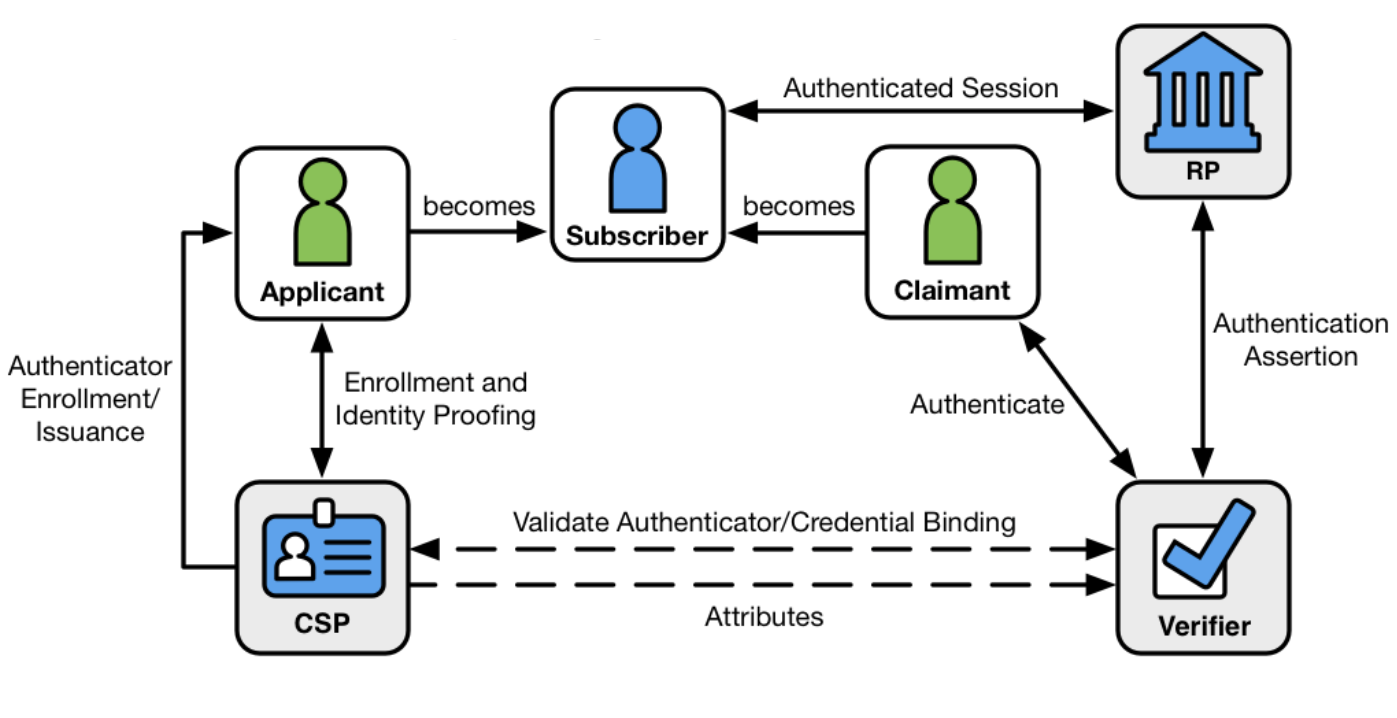
\includegraphics[width=13cm]{images/NIST_digital_identity_model}
	\caption{NITS Digital Identity Model}
	\label{fig:NIST-digital-identity-model}
\end{figure*}

\paragraph{Note on delegation of roles} %TODO: Italics
In the digital identity model \ref{fig:NIST-digital-identity-model} roles of CSP, verifier and RP are distinct in their responsibility. 
In practice however all these roles can be performed by a single party (e.g any website with native registration and login).

In OAuth2's \cite{hardt2012oauth} authentication layer, the resource owner has the roles of applicant, claimant and subscriber. The authorisation server has the roles of CSP and verifier. The OAuth2 client has the role of the RP. %TODO: Italics

\subsection{Authentication Factors}

As described in \cite{council2005authentication} authentication systems can rely on three distinct "factors".

\begin{itemize}
	\item \textbf{Knowledge factors} - Something the user \textbf{knows} (e.g, password, security question, PIN)
	\item \textbf{Ownership factors} - Something the user \textbf{owns} (e.g, ID card, security tokens, mobile devices)
	\item \textbf{Inherence factors} - Something the user \textbf{is} or \textbf{does} (e.g, static biometrics - fingerprints, retina, face. dynamic biometrics - voice patterns, typing rhythm)
\end{itemize}

\paragraph{Strong authentication} as defined by government and financial institutions is, an authentication procedure based two or more authentication factors. Authentication using two or more factors is also referred to as \textit{multi-factor authentication}. %TODO: Add source

\subsection{Password Based Authentication}

Passwords are one of the oldest forms of authentication, dating back to ancient times when it was used in the Roman military. It was first used in computers at MIT in the mid-60s \cite{mcmillan2012password}.

% High level arch
Password based authentication is a simple authentication model, based on a shared secret between a user and a system. The secret (password) is used in a combination with a user ID. Most common passwords are a set of characters and are memorised by the user.

Using NIST Digital Identity Guidelines terminology \cite{grassi2017}, the password and the user ID are issued as a credential and an authenticator to the applicant after successful enrolment by the CSP.
A claimant then uses the credentials to authenticate with the verifier, as to establish an authenticated session with the RP.


% Security considerations
\subsubsection{Security}

The simplicity of password-based authentication is also its downside, and the IT community has actively been working to move away from password based authentication and its downsides.
While there are many general attack vectors in any authentication system such as network conditions (man-in-the-middle) and the integrity of the system (viruses, key-loggers). The biggest risk specific to a password-based authentication system is choosing, handling and storing the passwords. %TODO: Review, expand, add sources

Passwords need to be memorised by the user, which creates an incentive for users to pick passwords that are shorter in length and contain less variance \cite{conklin2004password}. %TODO: Review

Ways in which adversaries can attack a PBS can be generally categories based on attackers access to "authenticator data", NIST \cite{grassi2017} classifies \textit{online} and \textit{offline} attacks as. %TODO: Rewrite according to passive/active attacks term + unauthorised access to database.

\paragraph{Online attack} An attack where the attacker assumes the role of the claimant with a genuine verifier.
A common type of attack is a \textit{guessing attack}, where and adversary repeatedly attempts to authenticate with the verifier by guessing possible passwords, this makes the attack very noisy and easy to detect and mitigate.


\paragraph{Offline attack} An attack where an attacker is able to analyse data in a system he controls. Data was obtained by the attacker by either theft of file, eavesdropping an authentication protocol or a system penetration.

Protecting against an offline attack means making it very expensive for an attacker to guess the password or "crack the password".
What influences the cost of guessing a password is the expected password entropy and the time to guess a single password.

\subparagraph{Password storage}
An important defence against offline attack are the methods with which passwords are stored and verified.
Trivially passwords stored in plaintext or hashed passwords are easy for an attacker to exploit efficiently with methods like pre-computed hash and rainbow tables. 

Modern password based security relies on methods of key-derivation that make password cracking both time-consuming and memory-hard \cite{percival2016scrypt, biryukov2016argon2, boneh2016balloon} and using \textit{salt} \cite{hornby2016salted} to make pre-computation attacks infeasible.
Key-derivation functions transform the plain text passwords into password hashes for storage.
When the system wants to verify a password it repeats the process of key-derivation and compares the output hash with the one in storage. %TODO: Expand more on available kdf functions.

\subparagraph{Password strength}
\textit{The strength} of a password directly relates to its entropy. The overall cost password cracking can be reduced by orders of magnitude by a week password, because the attacker has a smaller pool of passwords to try.
Have I Been Pwned \cite{hunt2021have} catalogs 613,584,248 passwords recovered from data breaches, while CrackStation \cite{hornby2019password} lists a collection of 1,493,677,782 words used for password cracking. Any password cracking software will exhaust the list in relatively short time compared to a brute-forcing technique.









\section{Extensible Authentication Protocol}

Extensible Authentication Protocol \cite{aboba2004extensible} (EAP) is a general purpose authentication framework, designed for network access authentication, where IP might not be available. 
It runs directly over the data link layer such as PPP  \cite{simpson1994rfc1661} and IEEE 802.

EAP defines a set of messages that support negotiation and execution of a variety of authentication protocols.

%EAP - PROTOCOL IN DETAIL

\subsection{Overview}
EAP is a two-party protocol between a \textit{peer} and an \textit{authenticator} at the each end of a link. In the protocol the peer is authenticating with the authenticator.

The protocol is initiated by the authenticator, by sending a \textit{Request} message to the peer, and the peer responds with a \textit{Response} message in a lock-step fashion. 
The success of the authentication is signalled  with a terminal \textit{Success} or \textit{Failure} message.

\subsection{Messages}

%TODO: EAP Packet with table

\paragraph{Request and Response} %TODO: Change Type to lowecase

Request messages are send from the authenticator to the peer.
Request packets have a Type field that indicates what is requested.
The peer processes the packet according to the Type field and send a Response of the same Type.
The Type of the Request determines the data in the packet.

\paragraph{Success and Failure} %TODO: Display field

After a successful completion of an authentication method an authenticator sends a Success packet to peer. A Failure packet is sent if the peer cannot be authenticated with the authenticator.

%EAP - METHODS

\subsection{Request Types}

The Type field of a Request packet indicates what information is being requested. First three types are special purpose types.

\subsubsection{Identity} \textbf{Type 1}. Used to query the identity of the peer.

\subsubsection{Notification} \textbf{Type 2}. Used to convey a message from the authenticator to the peer.

\subsubsection{Nak} \textbf{Type 3}. Used only as a response to a request, where the desired authentication type is not available.
The peer includes desired authentication methods, indicated by their type number.
This type is also referred to as Legacy Nak, when compared to Expanded Nak (sub-type of the Expanded Type).

\subsubsection{Expanded Type} \textbf{Type 254}. The Type field in the EAP packet is 1 octet long, and can represent 256 distinct values.% TODO: Add table representation
Expanded Types expand the space for available method types by adding a \textit{Vendor-ID} field (3 octets) and a \textit{Vendor-Type} (4 octets).

When a peer does not support the authentication method requested in an Expanded Type request it needs to respond with an Expanded Nak response. 
If the peer lack support for Expanded Types, it needs to respond with a Legacy Nak.

\subsubsection{Authentication Methods}
The remaining types correspond to different authentication methods.
According to IANA 49 authentication methods have been assigned Type numbers \cite{joseph2004eap}.

The original RFC \cite{aboba2004extensible} already assigned 3 authentication protocols.

\begin{itemize}
	\item \textbf{Type 4} - MD5-Challenge
	\item \textbf{Type 5} - One-Time Password
	\item \textbf{Type 6} - Generic Token Card
\end{itemize}

Some notable examples are EAP-TLS \cite{simon2008eap}, EAP-PSK \cite{bersani2007eap}, EAP SRP-SHA1 \cite{carlson135eap}. % TODO: Mention that EAP SRP is interesting as it is ZKP
The IANA list is not accounting for any authentication methods supported with the Expanded Type.

%EAP - USAGES

\subsection{Pass-Through Behaviour}
An authenticator can acts as a "Pass-Through Authenticator", relying on authentication services of a \textit{backend authentication server}. 
In this mode of operation the authenticator is relaying the EAP packets between the peer and the backend authentication server.

In IEEE 802.1x the authenticator communicates with a RADIUS server \cite{congdon2003ieee}.

\subsection{IEEE 802.1x}

IEEE 802.1x is standard for port based network access control for LAN and WLAN. It is part of the IEEE 802.11 group of network protocols.

IEEE 802.1x defines an encapsulation of EAP for use over IEEE 802 as EAPOL or "EAP over LANs".
%NOT clear if EAP used in WPA2-PSK
EAPOL is used in widely adopted wireless network security standards WPA2. In both WPA2-Personal and WPA2-Enterprise, EAPOL is used for communication between the supplicant (wireless station) and the authenticator (access point).

With WPA2-Enterprise, the authenticator (Access Point) functions in a pass-through mode as uses a RADIUS server for authentication services. 
EAP packets between the authenticator and the authentications server (RADIUS) are encapsulated as RADIUS messages \cite{aboba2003radius, chen2005extensible, congdon2003ieee}
\section{Password-based Authentication using Zero-Knowledge Proof of Quadratic Residues}

The original paper on zero-knowledge proofs outlined a zero-knowledge proof protocol based on the problem of quadratic residues.

\subsection{Protocol} %TODO: Restructure to focus soley on ZKPQR as PBA

Public inputs $n,x: (\frac{x}{n}) = 1$ and\\
Provers private input $w: x \equiv w^2 \Mod{n}$\\
\begin{center}
\begin{tabular}{rl}
	P $\rightarrow$ V: & Choose $u \leftarrow_R \Bbb{Z}_{n}^{*}$; Send $y = u^2$\\
	V $\rightarrow$ P: & Choose $b \leftarrow_R \{0, 1\} $; Send $b$\\
	P $\rightarrow$ V [$b = 0$]: & Send $u$\\
	P $\rightarrow$ V [$b = 1$]: & Send $z = w \cdot u \Mod{n}$\\
	V [$b = 0$]: & Check $z^2 \equiv y \Mod{n}$\\
	V [$b = 1$]: & Check $z^2 \equiv xy \Mod{n}$\\
\end{tabular}
\end{center}

This protocol is repeated $m$ times, for a confidence of $1 - 2^{-m}$.

% Security
\subsection{Security}

%TODO Maybe use passive/active attack terminology
\subsubsection{Offline Attacks}
The input $x$ is used by the Verifier to verify the proof, it is computed from the private input $w$ as $x = w^2 \Mod n$.
The $w$ is the Provers private input and represents the users password in a password-based authentication system.

The problem in an application of this protocols in the storage of $w$.
In modern password-based authentication system, the password is processed by a resource expensive password key derivation function, and the authentication is verified by comparing the derived values.
Our protocol prevents us from using key derivation in this way, because without the original or "plaintext" value $x$ we cannot verify the proofs provided by the Prover.

However storing the "plaintext" values of $x$, enables an attacker to easily pre-compute a table of possible $x$ values.

% Key derivation function
%TODO Pick a different title
\subsubsection{?? Client-Side Key Derivation}
Our wish is to use a hashing function with salt on the password and use the original value of $x$ for verification.
To achieve both requirements, the password is hashed before used to calculate the $x$ used for verification in the authentication process.
This approach is similar to the one used in \cite{wu1998secure} the Secure Remote Password protocol.
Using a hashing function $H$, a random salt $s$ and users password $P$, we can derive $w$ and $x$.

$$w = H(P, s)$$
$$x = w^2 \Mod n$$

\subsection{Protocol}
Using the NIST Digital Identity Guidelines \cite{grassi2017}.

\paragraph{Values}
\begin{center}
	\begin{tabular}{rl}
		$q, p$ & Primes, where $q \ne p$\\
		$n$ & Modulo number, where $n = qp$\\ %TODO check the correct term for this 
		$P$ & Provers password \\
		$I$ & Provers identifier \\
		$H$ & Hashing function \\
		$s$	& Salt\\
		$w$ & Password hash, where $w = H(P, s)$\\ %TODO check the correct term for this
		$x$ & Integer, where $x = w^2 \Mod{n}$ %TODO check the correct term for this
	\end{tabular}
\end{center}


\paragraph{Enrolment} In the enrolment process the CSP provides the $n$ modulo value to the Applicant.
The Applicant generates a random salt $s$ and computes a private $w$ value from the password $P$, $w = H(P, s)$.
Applicant next computes $x = w^2 \Mod{n}$ and submits the identifier $I$ and $x$ to the CSP.

\bigskip

\begin{center}
\begin{tabular}{rl}
	CSP $\rightarrow$ Ap: & Send $n$\\
	Ap: & Generate $s$\\
	Ap: & Compute $w = H(P, s)$\\
	Ap: & Compute $x = x^2 \Mod{n}$\\
	Ap $\rightarrow$ CSP: & Send $I, x, s$
\end{tabular}
\end{center}

\bigskip

%TODO Make sure this checks out.
CSP binds $x$ and $s$ as the authenticator to the credential $I$.

\paragraph{Authentication}

Authentication happens in two part, in the first part minimal data is exchanged between the Claimant and the Authenticator. The Claimant identifies himself and the Authenticator provides the $n$ and the salt $s$. %TODO Give $n$ a name
In the second part the protocol for ZKP of Quadratic Residuosity is executed between the Claimant and the Authenticator. %TODO Check spelling

To draw parallels between the terminology used in the ZKP of Quadratic Residuosity \cite{GMR} and the NIST Digital Identity Guidelines \cite{grassi2017}. The Prover is the Claimant, and the Verifier is the Authenticator.

\bigskip

\paragraph{First Part (Setup)}

The Claimant sends an identifier $I$ to the Authenticator, which responds with modulo $n$ and the salt $s$. The Claimant uses both values to compute the private input $w$ of the ZKPQR protocol.

\bigskip

\begin{center}
	\begin{tabular}{rl}
	C $\rightarrow$ Au: & Send $I$\\
	Au $\rightarrow$ C: & Send $n, s$\\
	C: & Computes $w = H(P, s)$\\
\end{tabular}
\end{center}

\paragraph{Second Part (ZKPQR)}
This part is same as the ZKPQR protocol described in the \cite{GMR}.

\bigskip

\begin{center}
\begin{tabular}{rl}
	C $\rightarrow$ Au: & Choose $u \leftarrow_R \Bbb{Z}_{n}^{*}$; Send $y = u^2$\\
	Au $\rightarrow$ C: & Choose $b \leftarrow_R \{0, 1\} $; Send $b$\\
	P $\rightarrow$ V [$b = 0$]: & Send $u$\\
	P $\rightarrow$ V [$b = 1$]: & Send $z = w \cdot u \Mod{n}$\\
	V [$b = 0$]: & Check $z^2 \equiv y \Mod{n}$\\
	V [$b = 1$]: & Check $z^2 \equiv xy \Mod{n}$\\
\end{tabular}
\end{center}

% Enrolment

% Authentication
\section{PBA Using ZKPQR Implemented as an EAP Method} %TODO: Reword every Sub-Type to Subtype
%TODO: Introduction, explain name

\subsection{EAP Packet Format}
An EAP packet is $n$ octets long.


\begin{center}
\begin{tabular}{|c|c|c|c|c|c|}
	\hline
	1 & 1 & 2 & 1 & 1 & $n - 6$\\
	\hline
	Code & Identifier & Length & Type & Sub-Type & Sub-Type Data\\
	\hline 
\end{tabular}
\end{center}

\paragraph{Code}
The code field is one octet

\bigskip

\begin{tabular}{ll}
	1 & Request \\
	2 & Response\\
\end{tabular}

\paragraph{Identifier} The identifier field is one octet, and is being used to match request and response packets.

\paragraph{Length} Two octets long, used to indicate the length of the EAP packet.

\paragraph{Type} One octet long.

\bigskip

\begin{tabular}{ll} %TODO: Change the sex joke
	69 & EAP PB-ZKP-QR \\
\end{tabular}

\paragraph{Subtype} One octet long

\bigskip 

\begin{tabular}{ll}
	1 & SETUP \\ %TODO: Better names
	2 & ZKP-QR \\
\end{tabular}

\subsubsection{Subtype 1 Request}

EAP Sub-Type 1 request must be sent after obtaining the peers identity. The identity can be acquired with the EAP-Identity (Type 1) packet, or determined somehow otherwise.

The peers identity is used to look up the password salt $s$ and modulus $n$.

\bigskip

\begin{center}
\begin{tabular}{|c|c|c|}
	\hline
	1 & $4 \le n \le 255 $ & $64 \le m$\\
	\hline
	Salt Length & Salt & Modulus\\
	\hline
\end{tabular}
\end{center}

\paragraph{Salt Length}
A single octet for the length of the Salt field in octets. %TODO: Maybe reword copied from EAP-SRP-RFC

\paragraph{Salt}
A random salt value, should be from 4 octets to 255 octets long.
The max length is determined by the max number able to be encoded in the Salt Length field.

\paragraph{Modulus}
Fills the rest of the message to the length specified by the Length field in the EAP header. %TODO: Maybe reword copied from EAP-SRP-RFC
Should be at least 64 octets (512 bits).

This is the $n$ value in the ZKR-QR protocol, a product of two primes $n = qp$.


\subsubsection{Subtype 1 Response}
The request of this subtype serves to complete the setup phase of the protocol, while the response already provides the $y$ value required at the start of each cycle of the second part of the protocol.

\begin{center}
\begin{tabular}{|c|}
	\hline
	$n$ \\
	\hline
	Square $y$\\
	\hline
\end{tabular}
\end{center}

\bigskip

\paragraph{Square $y$} Computed by the peer, as $y = u^2$, where $u \leftarrow_R \Bbb{Z}_{n}^{*}$. Fills the remainder of the message in $n$ octets.

\subsubsection{Subtype 2 Request}

\begin{center}
\begin{tabular}{|c|}
	\hline
	$1$ \\
	\hline
	Random Bit $b$\\
	\hline
\end{tabular}
\end{center}

\paragraph{Random Bit $b$} A single-bit, at the right-most place. The bit value is randomly chosen by the authenticator. 1 octet long.

\subsubsection{Subtype 2 Response}

\begin{center}
\begin{tabular}{|c|c|c|}
	\hline
	$1$ & $n \le 255 $ & $m$\\
	\hline
	Witness Length & Witness $z$ & Square $y$\\ %TODO: Witness, check if this is the correct term?
	\hline
\end{tabular}
\end{center}

\paragraph{Witness Length} A field one octet in length. Determines the length of the Witness field in octets.

\paragraph{Witness} Fields length is limited by the max value of the Witness Length field at 255 octets.
The witness $z$ is computed by the peer, the computation depends on the value of the random bit $b$ in the request.
If $b=0$, then $z = u$, where $u$ was generated for the subtype 1 response.
If $b=1$, then $z = w \cdot u$,  where $u$ was generated for the subtype 1 response, and $w$ is the provers private input.

\paragraph{Square $y$} Field fills up the remainder of the message. 
Square $y$ is the same value as in the subtype 1 response.
It is generated and sent in the $n$-th cycle, to help verify the witness in the $(n+1)$-th cycle.
Same rules apply as when generating the $y$ value if the response to subtype 1 request.

\subsection{Optimisations}
EAP is a lock-step protocol of request response pairs, each packet is first sent by the authenticator as a request, and the peer returns the message as a response. % TODO: Reword this

A naive mapping of ZKP-SQ messages to EAP packets yields 3 new Request/Response pairs. 
We can reduce the amount of new pairs to 2 instead of 3, by interlacing data shared in each pair.

This way we can obtain faster performance by reducing the number of packet needed needed to be exchanged.

\paragraph{Naive Map}

\begin{center}
	\begin{tabular}{c|rcl}
	Pair & Peer  & $\leftrightarrow$ & Authenticator \\
	\hline
	1 & & $\xleftarrow{\text{s, n}}$ &\\
	&& $\xrightarrow{\textvisiblespace}$&\\
	\hline
	2 & & $\xleftarrow{\textvisiblespace}$&\\
	&& $\xrightarrow{y}$&\\
	\hline
	3 & & $\xleftarrow{b}$&\\
	&& $\xrightarrow{z}$&\\
	\hline
	\end{tabular}
\end{center}

\subparagraph{Pair 1} Exchanged once after the authenticator obtaining the peers identity. The authenticator communicates the salt $s$ and modulus $n$ to the peer, in order for the peer to compute the private input $w$. 
Peers response serves as an acknowledgement of a successful setup.

This pair corresponds to the \textit{setup} part of the protocol.

\subparagraph{Pair 2} The authenticator requests the peer to generate the \textit{square} value $y$ and share it in the response.

This pair corresponds to the \textit{interactive zero-knowledge proof} part of the protocol and is repeated for $m$ times. 

\subparagraph{Pair 3} The authenticator requests the peer to compute the \textit{witness} value $z$, according to the procedure determined by the random bit $b$ in the request data.

This pair corresponds to the \textit{interactive zero-knowledge proof} part of the protocol and is repeated for $m$ times.

\subparagraph{Performance}
With this mapping a successful protocol run of $m$ iterations with a confidence of $1 - 2^{-m}$, would require a minimum of $4m + 3$ packet exchanges.

\bigskip

\begin{tabular}{r|l}
	Packets exchanged & Type\\
	\hline
	2 & Pair 1\\
	$2m$ & Pair 2\\
	$2m$ & Pair 3\\
	1 & Type 2 (Success)\\
\end{tabular}

\paragraph{Interlaced Data Mapping}

\begin{center}
	\begin{tabular}{c|rcl}
	Pair & Peer  & $\leftrightarrow$ & Authenticator \\
	\hline
	1 & & $\xleftarrow{\text{s, n}}$ &\\
	&& $\xrightarrow{y_1}$&\\
	\hline
	2 & & $\xleftarrow{b}$&\\
	&& $\xrightarrow{z, y_{n+1}}$&\\
	\hline
	\end{tabular}
\end{center}

\subparagraph{Pair 1} Exchanged once after the authenticator obtaining the peers identity. The authenticator communicates the salt $s$ and modulus $n$ to the peer, in order for the peer to compute the private input $w$. 
Peers computes the square value $y$ and sends it in the response.

The main difference with the naive mapping is that the peer responds prematurely with $y$, instead of in the response to naive pair 2. %TODO: Reword, weird sentence
Trivially we see, that it is possible and valid, because the modulus value $n$ is provided in the pair 1 request.

\subparagraph{Pair 2}
The authenticator already receiving the square value $y$ can send a request with a random bit $b$. The peer responds by computing the \textit{witness} $z$ according to $b$.
The peer also computes the square value $y_{n+1}$, which is used in the next iteration of the protocol.

This is possible because the computation of square value $y$ is only dependent on the modulus $n$, which is established in the request pair 1.

\subparagraph{Performance}
With this mapping a successful protocol run of $m$ rounds with an error rate $2^{-m}$, would require a minimum of $2m + 3$ packet exchanges.

Comparing the performance of both mappings, the interlaced mapping requires half as many exchanges for the same $m$ rounds of protocol.

$$\lim_{1 \rightarrow \infty} \frac{2x + 3}{4x + 3} = \frac{1}{2}$$

\bigskip

\begin{tabular}{r|l}
	Packets exchanged & Type\\
	\hline
	2 & Pair 1\\
	$2m$ & Pair 2\\
	1 & Type 2 (Success)\\
\end{tabular}

\subsection{Security}


%\subsection{Salt / Modulus Sub-Type Response Data Format}
%After the response is sent the first part of the protocol is successfully finished, and can move to the second part.
%The second part of the protocol is repeated for multiple times compared to the first part which only happens once. 
%
%A new $y$ value is required at the start of each iteration, for this reason it is always required in the subtype 2 response \ref{subtype-2-response}. The response \textbf{can} contain the value of $y$, required in the second part of the protocol, according to the data format defined in \ref{subtype-2-response}. 
%However the response can also be empty and serve only as an acknowledgment. %TODO: Badly worded
%
%\subsection{Send Y Sub-Type Request Data Format}
%This is initial request of an iteration of the second part of the protocol.
%The request is empty
%
%\subsection{Send Y Sub-Type Response Data Format}
%\label{subtype-2-response}
%
%\subsection{Send Z Sub-Type Data Format}
%
%\subsection{Send Z Sub-Type Data Format}






\bibliographystyle{alpha}

\bibliography{ref}

\end{document}